% This is based on "sig-alternate.tex" V1.9 April 2009
% This file should be compiled with V2.4 of "sig-alternate.cls" April 2009
%
\documentclass{report}

\usepackage[english]{babel}
\usepackage{graphicx}
\usepackage{tabularx}
\usepackage{subfigure}
\usepackage{enumitem}
\usepackage{url}


\usepackage{color}
\definecolor{orange}{rgb}{1,0.5,0}
\definecolor{lightgray}{rgb}{.9,.9,.9}
\definecolor{java_keyword}{rgb}{0.37, 0.08, 0.25}
\definecolor{java_string}{rgb}{0.06, 0.10, 0.98}
\definecolor{java_comment}{rgb}{0.12, 0.38, 0.18}
\definecolor{java_doc}{rgb}{0.25,0.35,0.75}

% code listings

\usepackage{listings}
\lstloadlanguages{Java}
\lstset{
	language=Java,
	basicstyle=\scriptsize\ttfamily,
	backgroundcolor=\color{lightgray},
	keywordstyle=\color{java_keyword}\bfseries,
	stringstyle=\color{java_string},
	commentstyle=\color{java_comment},
	morecomment=[s][\color{java_doc}]{/**}{*/},
	tabsize=2,
	showtabs=false,
	extendedchars=true,
	showstringspaces=false,
	showspaces=false,
	breaklines=true,
	numbers=left,
	numberstyle=\tiny,
	numbersep=6pt,
	xleftmargin=3pt,
	xrightmargin=3pt,
	framexleftmargin=3pt,
	framexrightmargin=3pt,
	captionpos=b
}

% Disable single lines at the start of a paragraph (Schusterjungen)

\clubpenalty = 10000

% Disable single lines at the end of a paragraph (Hurenkinder)

\widowpenalty = 10000
\displaywidowpenalty = 10000
 
% allows for colored, easy-to-find todos

\newcommand{\todo}[1]{\textsf{\textbf{\textcolor{orange}{[[#1]]}}}}

% consistent references: use these instead of \label and \ref

\newcommand{\lsec}[1]{\label{sec:#1}}
\newcommand{\lssec}[1]{\label{ssec:#1}}
\newcommand{\lfig}[1]{\label{fig:#1}}
\newcommand{\ltab}[1]{\label{tab:#1}}
\newcommand{\rsec}[1]{Section~\ref{sec:#1}}
\newcommand{\rssec}[1]{Section~\ref{ssec:#1}}
\newcommand{\rfig}[1]{Figure~\ref{fig:#1}}
\newcommand{\rtab}[1]{Table~\ref{tab:#1}}
\newcommand{\rlst}[1]{Listing~\ref{#1}}



%%% Our own commands
\newcommand{\name}{ReciPy\texttrademark}

% General information

\title{\name\\
\normalsize{Distributed Systems -- Project Proposal}}
\subtitle{subtitle}

% Use the \alignauthor commands to handle the names
% and affiliations for an 'aesthetic maximum' of six authors.

\numberofauthors{1} %  in this sample file, there are a *total*
% of EIGHT authors. SIX appear on the 'first-page' (for formatting
% reasons) and the remaining two appear in the \additionalauthors section.
%
\author{
% You can go ahead and credit any number of authors here,
% e.g. one 'row of three' or two rows (consisting of one row of three
% and a second row of one, two or three).
%
% The command \alignauthor (no curly braces needed) should
% precede each author name, affiliation/snail-mail address and
% e-mail address. Additionally, tag each line of
% affiliation/address with \affaddr, and tag the
% e-mail address with \email.
%
% 1st. author
\alignauthor \normalsize{Nintendo}\\
	\affaddr{\normalsize{69-666-007}}\\
	\email{\normalsize{awsum@sauce.com}}
}


\begin{document}

\maketitle

	\begin{abstract}
		Iz veeeeeeeeeeeeeeeeeeeeeeeeeery nyce...
	\end{abstract}

	\section{Introduction}

	\name iz dank af.

\section{System Overview}

We uz dem fones to do the stuffz.

And it workz!

\begin{figure}[h]
	\centering
    
\includegraphics[width=\columnwidth]{satisfied.jpeg}
	\caption{Pepe aprovez}
\end{figure}


\section{Requirements}
	
	You haz 2 B dis high to ride.
	
	\begin{figure}[h]
	\centering
    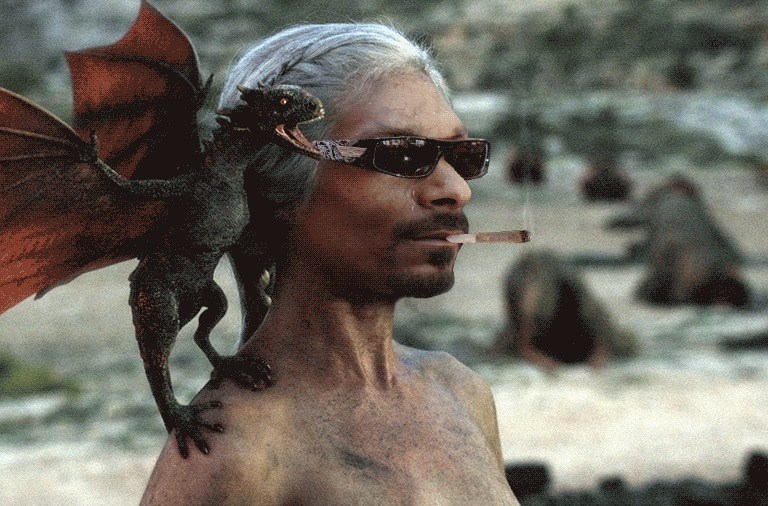
\includegraphics[width=\columnwidth]{high.jpg}
	\caption{Dis high.}
\end{figure}

\section{Work Packages}

	We will pay lil asians to code for us. 

\section{Milestones}

\begin{enumerate}
	\item Plan the shit.
	\item Do the shit.
	\item Use the shit.
	\item Sell the shit.
	\item Buy Gorilla with money.
	\item Take over world.
	\item Drunk text your ex.
	\item Wait... What are we talkin' about again ?
	\item get hyped. Like this guy.
\end{enumerate}

\begin{figure}[h]
	\centering
    
\includegraphics[width=\columnwidth]{danked.jpeg}
	\caption{He hyped}
\end{figure}

\end{document}
